\section{Verde Windrider}\label{verde-windrider}

Tags: NPC Creatore: Lorenzo

\section{Verde Windrider}\label{verde-windrider-1}

\begin{center}\rule{0.5\linewidth}{0.5pt}\end{center}

\begin{figure}
\centering
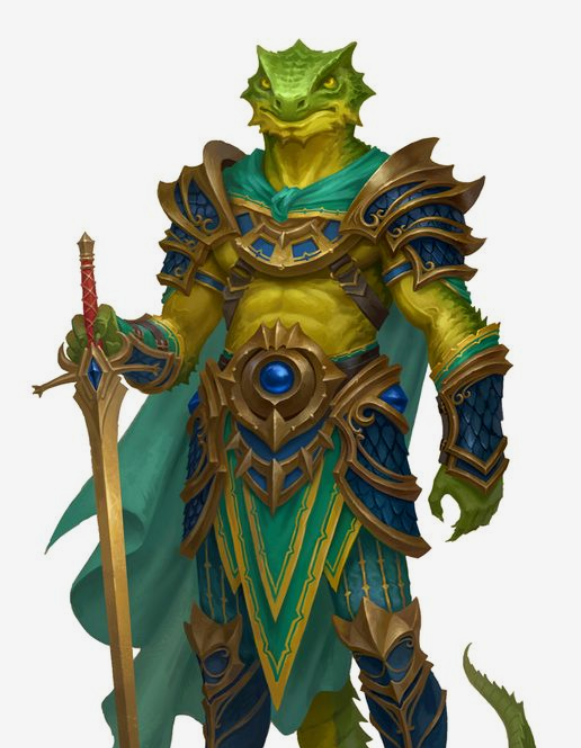
\includegraphics{Screenshot_2023-08-18_130011.png}
\caption{Screenshot 2023-08-18 130011.png}
\end{figure}

Informazioni Generali

Età: 45

Anno di nascita: 1978

Paese di nascita: ?

Razza: Lizardfolk

Relazioni: Paladino di San Francesco, Comandante Generale della Gilda
dei Protettori di Kos

Alleati: Ordine dei Paladini di San Francesco; Gilda dei Protettori
della Sila devoti a San Francesco e ai Lupi

Nemesi: Setta del Sangue

Possedimenti importanti:

\begin{center}\rule{0.5\linewidth}{0.5pt}\end{center}

\subsection{1. Descrizione Generale}\label{descrizione-generale}

\begin{center}\rule{0.5\linewidth}{0.5pt}\end{center}

Verde è un Lizard Folk dalla pelle squamosa di colore verde brillante,
che rispecchia il suo nome. Le sue scaglie sono resistenti e riflettono
la luce del sole in modo affascinante. Con un'altezza leggermente
superiore alla media per la sua razza, Verde emana un'aria di forza e
determinazione. La sua armatura da paladino, abbellita con simboli sacri
a San Francesco, brilla con luce propria, riflettendo la sua devozione
alla causa della giustizia.

\begin{quote}
``Custodire la luce della giustizia è un impegno che non conosce sosta,
un dovere che abbraccio con ogni scaglia del mio essere. Che il mio nome
sia ricordato come un protettore dei deboli e un difensore della
verità.''
\end{quote}

\subsection{2. Biografia}\label{biografia}

\begin{center}\rule{0.5\linewidth}{0.5pt}\end{center}

Durante una delle sue missioni, Sam, un paladino di San Francesco, trovò
un neonato di Lizard Folk abbandonato e in pericolo. Mosso a
compassione, decise di portarlo con sé e di allevarlo insieme a suo
figlio come se fossero fratelli. Gli diede il nome di Verde, a causa
delle sue scaglie di colore verde brillante. Verde crebbe forte e sano
sotto la cura del paladino, sviluppando un forte legame con suo fratello
adottivo Hart, che considerava il suo amico più intimo. Con il passare
degli anni, Sam addestrò entrambi i ragazzi alla vita di paladini. Essi
impararono le arti della guerra, ma anche l'importanza dell'empatia e
della compassione. Sam li istruì sulla natura degli spiriti elementali,
sull'importanza della preghiera e del rispetto della vita di ogni essere
vivente. Verde e Hart dimostrarono di essere molto talentuosi e
determinati, e quando il loro addestramento fu completato, giurarono
fedeltà a San Francesco come paladini, seguendo le orme del padre e
promettendo di servire la sua causa. Verde era grato a Sam per avergli
dato una famiglia e per avergli insegnato il significato della giustizia
e dell'onore. Il suo addestramento lo rese un paladino valoroso e
determinato, ma l'amicizia con Hart lo rendeva anche più umano e
compassionevole. Verde e suo fratello giurarono lo stesso mese del
Giorno del Sangue, momento più buio della storia dell'Ordine, in cui
molti nobili paladini, compreso Hart, persero la vita a causa del
tradimento dei loro compagni.

\subsection{3. Carriera}\label{carriera}

\begin{center}\rule{0.5\linewidth}{0.5pt}\end{center}

Verde ha dedicato gran parte della sua vita all'addestramento e alla
carriera di paladino. Dopo aver giurato fedeltà a San Francesco,
combatté con onore al fianco di suo padre Sam e dei paladini rimasti
nella la guerra del sangue. La sua tenacia e il suo coraggio
contribuirono alla vittoria dei paladini, vendicando la morte di suo
fratello adottivo Hart.

Dopo la guerra, Verde non si fermò. Insieme a un gruppo di paladini,
fondò la
\href{Gilda\%20dei\%20protettori\%20della\%20Sila\%20Devoti\%20a\%20San\%20Franc\%20e29bb7909af24fee931336355db913d4.md}{\textbf{Gilda
dei protettori della Sila Devoti a San Francesco e ai Lupi}} ,
un'organizzazione dedicata alla difesa dei deboli e alla promozione
della giustizia in tutto il mondo. Verde fu uno dei membri fondatori e
fece parte del primo Consiglio Supremo, noto come il Consiglio dei
Fondatori, che definì le basi della gilda.

Oggi, Verde è il Comandante Generale della sede della Gilda dei
Protettori a Kos, una posizione di grande responsabilità che lo vede
guidare la difesa della città e coordinare gli sforzi dei Protettori in
tutta la regione.

\subsection{4. Personalità}\label{personalituxe0}

\begin{center}\rule{0.5\linewidth}{0.5pt}\end{center}

Verde è noto per la sua natura compassionevole e la sua lealtà assoluta
ai principi di giustizia di San Francesco. Ha ereditato l'empatia e la
gentilezza di suo padre adottivo Sam, ma possiede anche la fermezza e la
determinazione di un paladino. È un individuo risoluto, sempre disposto
a proteggere gli indifesi e a combattere per ciò in cui crede.

La perdita di suo fratello adottivo Hart durante il Giorno del Sangue lo
ha spinto a impegnarsi ancora di più nella lotta contro le forze del
male. La sua personalità riflette una mescolanza di calma e
determinazione, rendendolo un comandante rispettato dai suoi uomini e un
paladino ammirato da coloro che protegge.

\subsection{A. Coinvolgimenti in eventi
recenti}\label{a.-coinvolgimenti-in-eventi-recenti}

\begin{center}\rule{0.5\linewidth}{0.5pt}\end{center}

\href{Untitled\%20Database\%2017d2e2b7db1d496f86b6dc2194d49887.csv}{Untitled
Database}

\subsection{B. Aggiornamenti}\label{b.-aggiornamenti}

\begin{center}\rule{0.5\linewidth}{0.5pt}\end{center}

\href{Untitled\%208c0a76f795b04cc580c646bb9b99fbb7.csv}{}
